\documentclass[english,12pt,a4paper,pdftex,sci,utf8]{./styles/aaltothesis}
\usepackage{graphicx}
\usepackage{ifpdf}
\ifpdf
   % put here packages only for the PDF:
   \DeclareGraphicsExtensions{.pdf,.png,.jpg,.mps}
   \usepackage{hyperref}
\else
   % put here packages only for the DVI:
\fi

% put all the other packages here:
\usepackage{./styles/clemens_thesis}

% \includeonly{./tex/preamble, ./tex/background }

\begin{document}

% !TEX root = ../thesis.tex

\university{Aalto University}
\school{School of Science}

\department{Department of Information and Computer Science}
\professorship{Machine Learning, Data Mining, and Probabilistic Modeling}

\univdegree{MSc}

\author{Clemens Westrup}

%% Your thesis title comes here and again before a possible abstract.
%% If the title is very long and latex does an
%% unsatisfactory job of breaking the lines, you will have to force a
%% linebreak with the \\ control character.
%% Do not hyphenate titles.
%%
\thesistitle{Awesomeness with job ads}

\place{Espoo}

\date{16.1.2015}

%% B.Sc. or M.Sc. thesis supervisor
%% Note the "\" after the comma. This forces the following space to be
%% a normal interword space, not the space that starts a new sentence.
%% This is done because the fullstop isn't the end of the sentence that
%% should be followed by a slightly longer space but is to be followed
%% by a regular space.
%%
\supervisor{Michael Mathioudakis, Ph.D.}

%% B.Sc. or M.Sc. thesis advisors(s). You can give upto two advisors in
%% this template. Check with your supervisor how many official advisors
%% you can have.
%%
\advisor{Prof.\ Aristides Gionis}
%\advisor{M.Sc.\ Polli Pohjaaja}

%% Aalto logo: syntax:
%% \uselogo{aaltoRed|aaltoBlue|aaltoYellow|aaltoGray|aaltoGrayScale}{?|!|''}
%%
%% Logo language is set to be the same as the document language.
\uselogo{aaltoYellow}{!}

%% Create the coverpage
%%
\makecoverpage


%% English abstract.
%% All the information required in the abstract (your name, thesis title, etc.)
%% is used as specified above.
%% Specify keywords
%%
%%
\keywords{NLP, bla bla, keyword}
%% Abstract text
\begin{abstractpage}[english]
  Your abstract in English. Try to keep the abstract short; approximately
  100 words should be enough. The abstract explains your research topic,
  the methods you have used, and the results you obtained.
  Your abstract in English. Try to keep the abstract short; approximately
  100 words should be enough. The abstract explains your research topic,
  the methods you have used, and the results you obtained.

  Your abstract in English. Try to keep the abstract short; approximately
  100 words should be enough. The abstract explains your research topic,
  the methods you have used, and the results you obtained.
  Your abstract in English. Try to keep the abstract short; approximately
  100 words should be enough. The abstract explains your research topic,
  the methods you have used, and the results you obtained.
\end{abstractpage}

%% Force a new page so that the possible English abstract starts on a new page
\newpage


%% Preface
\mysection{Preface}
I want to thank bla bla bla
\\

\vspace{5cm}
Otaniemi, 16.1.2015

\vspace{5mm}
{\hfill Clemens Westrup \hspace{1cm}}

%% Force new page after preface
%%
%% Pakotetaan varmuuden vuoksi esipuheen j�lkeinen osa
%% alkamaan uudelta sivulta
\newpage


%% Table of contents.
\thesistableofcontents


%% Symbols and abbreviations
\mysection{Symbols and abbreviations}

\subsection*{Symbols}

\begin{tabular}{ll}
$\mathbf{B}$  & magnetic flux density  \\
$c$              & speed of light in vacuum $\approx 3\times10^8$ [m/s]\\
$\omega_{\mathrm{D}}$    & Debye frequency \\
$\omega_{\mathrm{latt}}$ & average phonon frequency of lattice \\
$\uparrow$       & electron spin direction up\\
$\downarrow$     & electron spin direction down
\end{tabular}

\subsection*{Operators}

\begin{tabular}{ll}
$\nabla \times \mathbf{A}$              & curl of vectorin $\mathbf{A}$\\
$\displaystyle\frac{\mbox{d}}{\mbox{d} t}$ & derivative with respect to
variable $t$\\[3mm]
$\displaystyle\frac{\partial}{\partial t}$  & partial derivative with respect
to variable $t$ \\[3mm]
$\sum_i $                       & sum over index $i$\\
$\mathbf{A} \cdot \mathbf{B}$    & dot product of vectors $\mathbf{A}$ and
$\mathbf{B}$
\end{tabular}

\subsection*{Abbreviations}

\begin{tabular}{ll}
AC         & alternating current \\
APLAC      & an object-oriented analog circuit simulator and design tool \\
           & (originally Analysis Program for Linear Active Circuits) \\
BCS        & Bardeen-Cooper-Schrieffer \\ %% dash between the names
DC         & direct current \\
TEM        & transverse eletromagnetic
\end{tabular}


%% Tweaks the page numbering to meet the requirement of the thesis format:
%% Begin the pagenumbering in Arabian numerals (and leave the first page
%% of the text body empty, see \thispagestyle{empty} below).
%% Additionally, force the actual text to begin on a new page with the
%% \clearpage command.
%% \clearpage is similar to \newpage, but it also flushes the floats (figures
%% and tables).
%% There is no need to change these
%%
\cleardoublepage
\storeinipagenumber
\pagenumbering{arabic}
\setcounter{page}{1}


\listoftodos

%\maketitle
%\tableofcontents
%\listoffigures
%\listoftables

%% Content
% !TEX root = ../thesis.tex
% !TEX spellcheck = en-US

%% Leave first page empty
\thispagestyle{empty}

% - what (problem statement)
% - why (need statement)
% - how (approach)
% - related
% - results

\section{Introduction}

Language is one of the most complex behaviors our species has developed. We humans use it to efficiently transport knowledge between individuals and communicate even the most abstract concepts with it. It takes children years to learn to learn express their thoughts and the subtle nuances of one's language give a glimpse one's cultural environment and upbringing, one's emotional state and one's intellect.

Not surprisingly in the field of \gls{AI} and especially \gls{ML} building computer systems with linguistic capabilities and solving language-based problems poses one of the hardest challenges and has motivated decades of research in Computational Linguistics. In fact many of the famous test for universal machine intelligence are based on linguistic capabilities, among them the famous \emph{Turing test} by~\cite{Turing:1950aa} where the task is for a human judge to determine whether he is having a conversation with a human or a machine in order to determine if the machine can be called intelligent, or the \emph{compression test} proposed by~\cite{Mahoney:1999aa}, where a human's and machine's capability to predict missing words given a context is tested.

This thesis explores the specific task of predicting the semantic structure of job advertisements as a specific example of such a language-based task that turns out to be difficult even for humans to do.

% The title of this work ``An \emph{Exploration} of \emph{Recent Connectionist Advances} for \emph{Supervised Topic Prediction in Job Advertisements}'' can be broken down into three pieces that captures the essence of it:
%
% \begin{itemize}
%   \item Exploration: The nature of this work is explorative in 2 ways: First a problem has been researched to find well-defined and well-motivated application of machine learning on job advertisement data. Second a solution space was explored approach this problem with special emphasis at recent progress in research.
%   \item Recent Connectionist Advances: The work
% \end{itemize}


The work was done in close collaboration with the Helsinki-based media and learning company \emph{Sanoma}\footnote{\textquote{Sanoma is a front running consumer media and learning company in Europe. In Finland and the Netherlands we are the market leading media company with a broad presence across multiple platforms. In Belgium we are among the Top 5. Our main markets in learning are Belgium, Finland, the Netherlands, Poland and Sweden. We entertain, inform, educate and inspire millions of people every day. We employ some 7,500 professional employees operating in Europe.}, Source: \url{http://www.sanoma.com/en/who-we-are}, visited 06.06.2016} and the research motivation was thus constantly tied back into real world challenges in the scope of Sanoma's business needs.

\subsection{Problem Statement}

The problem addressed during with this thesis to better understand the structure of job advertisements. In particular job postings typically consist of several parts with a certain function or theme: Usually the company is introduced, the job is described with it's tasks and responsibilities, the requirements for the job are listed, then benefits and offerings by the company are named and the reader is asked to apply in a specified way he or she is interested.
Almost all of the text of a job description falls into these categories\footnote{Only about 4\% of the sentences collected for evaluating the final experiments in this thesis were sorted into the category \emph{other} while the rest falls into either of the categories described. This is described in more detail in Section~\ref{subs:Multi-class Sentence Classification}} and the task can thus be posed as predicting a category for each sentence in a job advertisement, that corresponds with this sentence belonging to one of the job ads' parts as described above.
This is a challenging problem in itself but can further be used to extract certain functional parts of each job ad, to study a possible correlation between structural patterns and the reach and success of an ad and so forth. The problem therefore can be labelled as \emph{Text Categorization} or \emph{Text Classification} as referred to in the scientific literature.


\subsection{Need Statement and Motivation}

% -- need statement

Today's media and education, the basis of Sanoma's core businesses, are undergoing drastic and fundamental transformations that are currently disrupting whole industries. Usage of digital media as a source of information has long surpassed print media. Sanoma's most well-known product, Finland's biggest daily newspaper \emph{Helsingin Sanomat}, lost 6\% of its circulation only in 2015\footnote{Source: http://www.digitalnewsreport.org/survey/2016/finland-2016/, visited 27.07.2016}, while the wide-spread use of social media challenges traditional ways we access information. Similarly in the field of education, with the rise of Massive open online course (MOOCs), traditional learning settings are challenged and the need for advanced techniques for data processing and analysis increases, e.g.\ to personalize and adapt the learning experience to each individual user and at the same time identify trends across large groups of learners to better meet the needs of education.

Sanoma provides a recruitment platform named \emph{Oikotie Työpaikat}. The service is in direct competition several other international players in the recruitment industry. Through this and other services Sanoma's collects large amounts of user-generated data, offering the potential to be leveraged for machine learning solutions to provide value for their users and innovate and enrich the company's offerings.
This was the company's initial motivation for this thesis project --- To explore ways to leverage user-generated data to potentially.

% -- research motivation

% -- personal motivation

From a personal perspective this work was interesting as offered many research possibilities while at the same time being relevant for and inspired by real life applications. The complex nature of \acrlong{CL} with its proximity to the general study of machine intelligence and the high interpretability of problems makes poses makes it a fascinating problem domain. This presented a great challenge to learn balancing scientific research objectives and yet exploring potential business and user needs, learn on new fronts and deepen the knowledge in others and apply it to real data.

\subsection{Related work}
\label{sub:Related work}

The problem of \gls{TC}, also known as Text Categorization, is one of the various challenges in the thriving fields of \acrfull{CL} and \gls{NLP}. These areas of research have started out as theoretically challenging but rather marginally popular fields between \acrfull{AI} and formal linguistics and have since exploded in terms of interest with their applications being deployed currently at large scale to practically all kinds of consumer products such as smart phones and home entertainment systems as well as digital services like social networks, automatic translation engines and conversational agents.
Today there are textbooks dedicated specifically to this area, such as~\cite{Manning:1999aa},~\cite{Jurafsky:2014aa} and~\cite{Clark:2013aa} There is also much overlap to the field of \gls{IR} that rose to popularity during the late 1980's due to the Internet starting to become a mainstream medium (see~\cite{Manning:2008aa},~\cite{Leskovec:2014aa} and the classic work by~\cite{Rijsbergen:1979aa}).

\subsubsection*{Syntactics, Semantics, and Pragmatics}
\label{subs:Vogues in NLP: Syntactics, Semantics, and Pragmatics}

The field of Natural Language Processing has undergone different trends of modeling approaches to tackle its challenges.~\cite{Cambria:2014aa} identify these as three main trend curves focusing on \emph{Syntactics}, \emph{Semantics}, and \emph{Pragmatics}. According to the authors the first trend of syntax-centered NLP is still prevalent and is based on algorithms that more or less directly operate on the words found in the processed texts.
The second trend operates on the semantics of text, thus being able to potentially tackle more challenging problems by addressing increasingly subtle notions of meaning and context. According to the author these types of approaches are still in the early phase but at the verge of being adapted by a broader audience of researchers and practitioners in the field.
The last trend curve of pragmatics regards the yet more complex issue of modeling inherent narratives in language where so far only pioneering work has been done but which, according to the authors, will lead to tackling problems of natural language understanding.

\subsubsection*{The Text Classification Problem}
\label{subs:The Text Classification Problem}

The problem of \acrfull{TC} specifically has seen many evolving fashions of approaches and more or less loosely follows the three trend curves described above. \gls{TC} has been of immense interest for several decades now due to the exponentially increasing amounts of text data being recorded in forms of e.g.\ user generated content through social networks and through the increased digitalization of our daily lives. Its applications reach from document filtering, automated metadata generation such as language classification to automatic email labeling, spam identification and sentiment detection, amongst others.

\acrlong{TC} is nowadays covered in standard works of \acrlong{IR} and \acrlong{ML}, such as~\cite{Manning:2008aa}. As~\cite{Sebastiani:2002aa} points out it is important to mention that the term \emph{automatic text classification} has also been used referring to different problems: \textquote{Aside from (i) the automatic assignment of documents to a predefined set of categories [\ldots], the term has also been used to mean (ii) the automatic identification of such a set of categories (e.g.,~\cite{Borko:1963aa}), or (iii) the automatic identification of such a set of categories and the grouping of documents under them (e.g.,~\cite{Merkl:1998aa}), a task usually called text clustering, or (iv) any activity of placing text items into groups, a task that has thus both TC and text clustering as particular instances~\cite{Manning:1999aa}}

\subsubsection*{Early Work and Syntactic Approaches}
\label{subs:Early Work and Syntactic Approaches}

Early approaches towards solving \acrlong{TC} tasks in the 1980's were in often based on expert systems consisting of sets of manually created logical rules, deciding upon the category of a text segment if a certain formula applies. As discussed by~\cite{Sebastiani:2002aa} the biggest downside is known as the \emph{knowledge acquisition bottleneck} which refers to the fact that each rule has to be manually created. In the 1980's machine \acrfull{ML} became more common where a \emph{classifier} automatically learns the attributes of the data and its association with the given data labels using a model that allows to then infer the categories for unseen data. This setting is called \gls{Supervised Learning} as labels for the data are given and predicted.

\acrshort{ML} approaches have since been developed in countless variations. As described earlier syntax-based approaches are still very common and most follow a classic pipeline of \emph{feature extraction} or \emph{indexing} of documents followed by \emph{inductive construction} of a classifier that is lastly evaluated by a measure of effectiveness. A very successful approach to feature extraction has been the introduction of N-Gram based models, also called \emph{bag-of-words} models, which that are based on word-cooccurrence frequencies of the terms that are present in the data (see Section~\ref{subs:N-gram Models (Methods)} for an introduction).
As~\cite{Mikolov:2012aa} explains \textquote{the most significant advantages of models based on n-gram statistics are speed (probabilities of n-grams are stored in precomputed tables), reliability coming from simplicity, and generality (models can be applied to any domain or language effortlessly, as long as there exists some training data). N-gram models are today still considered as state of the art not because there are no better techniques, but because those better techniques are computationally much more complex, and provide just marginal improvements, not critical for success of given application.}
The limitation of such models is that their statistics are directly based on word co-occurrences and thus exponentially increase in size as the desired context to be captured is expanded, making them infeasible to adapt to longer text sequences.

\subsubsection*{Semantic Approaches and Representation Learning}
\label{subs:Semantic Approaches and Representation Learning}

Recently approaches from the field of \emph{Representation Learning}, have found their way into and gained tremendous traction in the \gls{NLP} research community. Traditional techniques such as N-gram models, now also referred to as \gls{Feature Engineering} approaches, use prior domain or expert knowledge in order to build data representations that are effective in combination with a classifier. But as~\cite{Bengio:2013aa} point out this is a laborious and time-consuming task that only exposes the weakness from a Machine Learning point of view by not automatically learning such representations --- a challenge representation learning aims to address. Beyond that, with regards to \gls{CL} problems, most \gls{Feature Engineering} techniques do not capture well the semantics of language.

One example particularly popular method called \emph{word2vec} was introduced by \cite{Mikolov:2013ad} and learns word representation vectors, so-called \emph{word embeddings}, through a context-prediction task. This produces extremely rich representations capturing many subtleties in the layers of meaning of words\cite{Mikolov:2013ab}. Another approach related to \gls{Representation Learning} under the name of Transfer Learning has been proposed by~\cite{Do:2006aa}. Similarly, in attempts to find more expressive ways of modeling semantics of language several breakthrough achievements in \acrshort{NLP} have been made using various \gls{Deep Learning} based methods --- a related trend that the field has picked up.
\cite{Collobert:2011aa} succesfully applied a \acrfull{CNN} architecture to a number of standard problems in \gls{NLP} with the intention of minimizing the domain knowledge introduced: \textquote{The design of this system was determined by our desire to avoid task-specific engineering as much as possible. Instead we rely on very large unlabeled datasets and let the training algorithm discover internal representations that prove useful for all the tasks of interest.}.
Later~\cite{Kim:2014aa} improved the method slightly, improving on state-of-the-art results in 4 out of 7 of these standard problems. Numerous related work was done building on similar ideas, such as using a \acrshort{CNN} on character level resolution for \gls{TC}~\cite{Zhang:2015aa}, Multitask Learning and Semi-Supervised Learning to improve the generalization of the shared tasks\cite{Collobert:2008aa} and using \glspl{RNN}~\cite{Liu:2016aa}. Just recently facebook research released a tool called \emph{fastText}\footnote{The tool is publicly available on \gls{GitHub}: \url{https://github.com/facebookresearch/fastText}} for \gls{TC} with a focus fast run-time while still achieving close to state-of-the-art results. The related publications draw heavily on previous work on word embeddings and similar techniques (see~\cite{Joulin:2016aa} and~\cite{Bojanowski:2016aa}).

\subsubsection*{Further Related Work and Focus of This Thesis}
\label{subs:Further Related Work and Focus of This Thesis}

Numerous other classes of approaches exist and have been explored with varying popularity such as \gls{TC} using String Kernels~\cite{Lodhi:2002aa}, \gls{EM}~\cite{Nigam:2000aa} and\cite{McCallum:1999aa}, \gls{SOM}~\cite{Merkl:1998aa} and using a \gls{CRF} for sequence labeing~\cite{Lafferty:2001aa}.
Also problem areas from the field of \gls{Unsupervised Learning} are related with techniques such as~\gls{LDA} \cite{Blei:2003aa} for \gls{Topic Modeling} where labels for text documents are found without providing a \gls{Ground Truth} beforehand. However this work specifically focuses on comparing traditional syntactic approaches to more recent semantic ones, focusing on ideas from \gls{Representation Learning} and \gls{Deep Learning}, in particular \glspl{RNN}.

\subsection{Research Scope and Objectives}
\label{sub:Research Scope and Objectives}

This thesis was initiated as a research project for Sanoma's recruitment platform \emph{Oikotie Työpaikat} with the intention of exploring interesting and novel ways to use the various data generated through the use of this service. The research objectives were stated as follows:

\blockquote{Find an application of data mining / machine learning to the customer-generated data on the recruitment platform Oikotie Työpaikat which has the potential of bringing value to the user of the platform and is technically feasible in the scope of a master’s thesis. Further define and investigate a research problem that is essential to this application by researching literature and previous work on similar problems trying different approaches based on the literature using the results and learnings to create an improved approach.}

In order to meet these objectives a predefined development process was applied that will be explained in the next section.

\subsection{Methodological Approach}
\label{sub:Methodological Approach}

\begin{figure}[h]
    \centering
    \includegraphics[width=\textwidth]{img/double-diamond.pdf}
    \caption{Design process for this thesis, adapted from the \emph{Double Diamond Process} developed by the British Design Council (see~\cite{Council:2007aa})}
\label{fig:double-diamond}
\end{figure}

The development process for this thesis project was adapted from the Double Diamond design process developed by the by the British Design Council in 2005 (see ~\cite{Council:2007aa}). A design process is \textquote{the specific series of events, actions or methods by which a procedure or set of procedures are followed, in order to achieve an intended purpose, goal or outcome.}~\cite{Best:2006aa}.
The Double Diamond process consists of iterative, explorative learning phases where first a problem worth solving is found within the \emph{Problem Scope} and afterwards the best solution is formed in the \emph{Solution Scope}. Both scopes are navigated through a so-called divergence phase where the space explored for finding possibilities followed by a convergence phase where the options are reduced and combined. These phases, as illustrated in Figure~\ref{fig:double-diamond}, are called \emph{Discovery Phase} and \emph{Definition Phase} in the Problem Scope and \emph{Development Phase} and \emph{Delivery Phase} in the Solution Scope and briefly described next:

\paragraph{Discovery Phase}
\label{par:Discovery Phase}
In the Discovery Phase opportunities for problems worth solving are evaluated. Often their potential is measured in terms of economic impact (financial viability), attractiveness to and impact on users (desirability) and the level of technological challenge (feasibility).
These aspects require different ways of testing and as the priority in this work lays on primarily on evaluating the technical challenge the main tools were prototyping, technical benchmarking and literature research.

\paragraph{Definition Phase}
\label{par:Definition Phase}
The aim of the Definition Phase is to compile the learnings from the Discovery Phase and find the problem that has the most potential and will be tackled. This is done by iteratively reframing the problem and testing the implications of this definition.
Thus the final problem definition is often not simply selected but developed through a series of steps of refining the problem, testing and learning.

\paragraph{Development Phase}
\label{par:Development Phase}
When the final problem definition has been set the Development Phase aims to produce a wide variety of potential approaches to solving this problem. Here existing approaches are benchmarked and tested, and combined with new ideas, again through a \emph{test, learn, rescope} cycle.
With regards to this work literature research was combined with testing of various methods and evaluating there performance to learn which approaches work best and how they could be improved, combined or built upon.

\paragraph{Delivery Phase}
\label{par:Delivery Phase}
During the Delivery Phase the best possible solution is chosen through refinement of the different approaches that were evaluated. At the end there stands a result of the whole process, in this case a comprehensive evaluation and conclusion on the approaches.


\subsection{Results}



\subsection{Structure of the Thesis}

\begin{figure}[h]
    \centering
    \includegraphics[width=\textwidth]{img/double-diamond-with-structure}
    \caption{Structure of this thesis mapped to the \emph{Double Diamond Process} design process }
\label{fig:double-diamond-with-structure}
\end{figure}

The first section of this thesis gave a brief introduction into the topic of this work, outlined the motivation and the research problem approached and showed the research objectives, the scope of the thesis as well as related work.

% !TEX root = ../thesis.tex
% !TEX spellcheck = en-US

%% In a thesis, every section starts a new page, hence \clearpage
\clearpage

\section{Exploration}
\label{sec:Exploration}

This chapter will outline how with initial objectives and how I went all the way from an initial project start with exploration over collecting data and iterating the problem framing to learn from about the problem to designing the final task and collecting an appropriate dataset including quality control in a crowdsourced fashion. \todo{rewrite when chapter is done}

\subsection{Research Objectives}
\label{sub:Research Objectives}

This thesis was initiated as a research project for Sanoma's recruitment platform \emph{Oikotie Työpaikat} with the intention of exploring interesting and novel ways to use the various data generated through the use of this service. The research objectives were stated as follows:

\blockquote{Find an application of data mining / machine learning to the customer-generated data on the recruitment platform Oikotie Työpaikat which has the potential of bringing value to the user of the platform and is technically feasible in the scope of a master’s thesis. Further define and investigate a research problem that is essential to this application by researching literature and previous work on similar problems trying different approaches based on the literature using the results and learnings to create an improved approach.}


% --------

\subsection{Methodological Approach}
\label{sub:Methodological Approach}

\begin{figure}[h]
    \centering
    \includegraphics[width=\textwidth]{img/double-diamond.pdf}
    \caption{Design process for this thesis, adapted from the \emph{Double Diamond Process} developed by the British Design Council (see~\cite{Council:2007aa})}
\label{fig:double-diamond}
\end{figure}

The design and development process of the project was adapted from the double diamond approach that was developed by the by the British Design Council in 2005 (see ~\cite{Council:2007aa}). A design process is \textquote{the specific series of events, actions or methods by which a procedure or set of procedures are followed, in order to achieve an intended purpose, goal or outcome.}~\cite{Best:2006aa}.

\paragraph{Discover}
\label{par:Discover}

In the first stage of the project an initial idea, motivation or inspiration is given.

- prototyping
- interviews
- market research
-





- double diamond approach
- initial exploration of topics
- topic decision for structured text prediction
- design choice for fixing chunks (making it a supervised multi-class prediction)
- explorative data collection
- learnings and design choice for 6 mutually exclusive labels + sentence as atomic unit => final problem setting
- dataset collection through crowdflower with iterations







% - brief
% - given data
% - interest?
% - approach
% - found problem: predicting audience and popularity of job ads
% - in order to do so: learn about structure of job ads
% - problem setting as supervised task,
% - get data by free collection:
%   - to predict paragraphs
%   - to learn about how humans interpret and carry out this task
% - experiments: grouping tags automatically vs manually
% - predicting with tf.idf
% - reading up on how to write good job ads
% - can be grouped into 6 categories
% - framed as new mulit-class problem and setting up data collection
% - results: distribution and statistics, most of the data can somewhat go into these categories (other is the smallest amount)
% - then trying to evaluate the best method or combination of methods



\subsection{Approach}
\label{sub:Approach}

\subsection{data sections}
\label{sub:data sections}

% # personnel selection
% \cite{Chien:2008aa} - improving personnel selection with data mining
% \cite{Saidi-Mehrabad:2007aa} - The development of an expert system for effective selection and appointment of the jobs applicants in human resource management.
% \cite{Hokey-Min:2003aa} - Developing the profiles of truck drivers for their successful recruitment and retention: A data mining approach.
% \cite{Youyou:2015aa} - Computer-based personality judgments are more accurate than those made by humans
%
% # careers
% \cite{Shahaf:2012aa} - metro maps of science
%
% # formal vs informal language
% \cite{Faruqui:2011aa} - I Thou Thee, Thou Traitor": Predicting Formal vs. Informal Address in English Literature.
% \cite{Brooke:2014aa} -  Computational Approaches to Style and the Lexicon
%
% \cite{Lee:2015:RJO:2700171.2791048} - On Recommending Job Openings
%
% \cite{Luhn:1958aa} - A Business Intelligence System


\subsubsection{Explorative Paragraph Dataset1}

\todo{Picture of software setup?}

To collect first data a tool was build, consisting of a Node.js\footnote{[\ldots] Node.js is an open-source, cross-platform runtime environment for developing server-side Web applications. \url{https://nodejs.org/}} server using MongoDB\footnote{\textquote{MongoDB is a free and open-source cross-platform document-oriented database [\ldots].} Source: \url{https://en.wikipedia.org/wiki/Node.js}, Website: \url{https://www.mongodb.com}} as a database and communicating via a JSON with a simple website front-end using the mustache template engine\footnote{\textquote{Mustache is a simple web template system.} Source: \url{https://en.wikipedia.org/wiki/Mustache_(template_system)}, Website: \url{https://mustache.github.io}}.
The tool is online\footnote{\url{http://thesis.cwestrup.de/jobad-tagger/}} and it's source code is publicly available on GitHub\footnote{\url{https://github.com/cle-ment/thesis-tagger}} with it's API documentation hosted online as well\footnote{\url{http://thesis.cwestrup.de/jobad-tagger/apidoc/}}.

The data generated by using the free-form text description of each job ad and splitting it into paragraphs as can be seen in the software package as well\footnote{\url{https://github.com/cle-ment/thesis-tagger/blob/master/pre-processing.ipynb}}.

The goal of this prototype tool for data collection was on the one hand to acquire data in order to carry our first experiments as fast as possible, and on the other hand to gain a deeper understanding about the research problem itself by giving an open, unbiased task to the participants. In particular the question at hand was how humans label the content of the different parts of a job ad.

The exact task given to the participants was ``Describe what each section is about by adding one or more tags/keywords to it''. They were shown a job ad that was split into paragraphs and besides each paragraph was a text field to enter 1 or more tags.

\begin{figure}[h]
  \centering
  \includegraphics[width=\textwidth]{img/thesis-tagger-interface.png}
  \caption{Screen capture of the interface of the tagging tool}
\label{fig:thesis-tagger-interface}
\end{figure}

In a first step the tool was only shown to 3 participants to get immediate feedback if the user interface had flaws and whether the task was understood.   Based on this feedback the tool was improved by providing an example for the participants and then tested with a slightly larger group of 12 persons. After correcting a few minor details in the user interface a public link was then shared via social media and other channels with as many people as possible. A few days later the tool was then also shared internally within Sanoma where it was set up as a competition to tag the most possible job ads.

In total 91 job ads were tagged, resulting in 379 tagged text sections and 358 tags.

\todo{Describe data: Different characteristics}
\todo{show distribution?}
\todo{show embedding visualizations}

\begin{figure}[h]
    \centering
    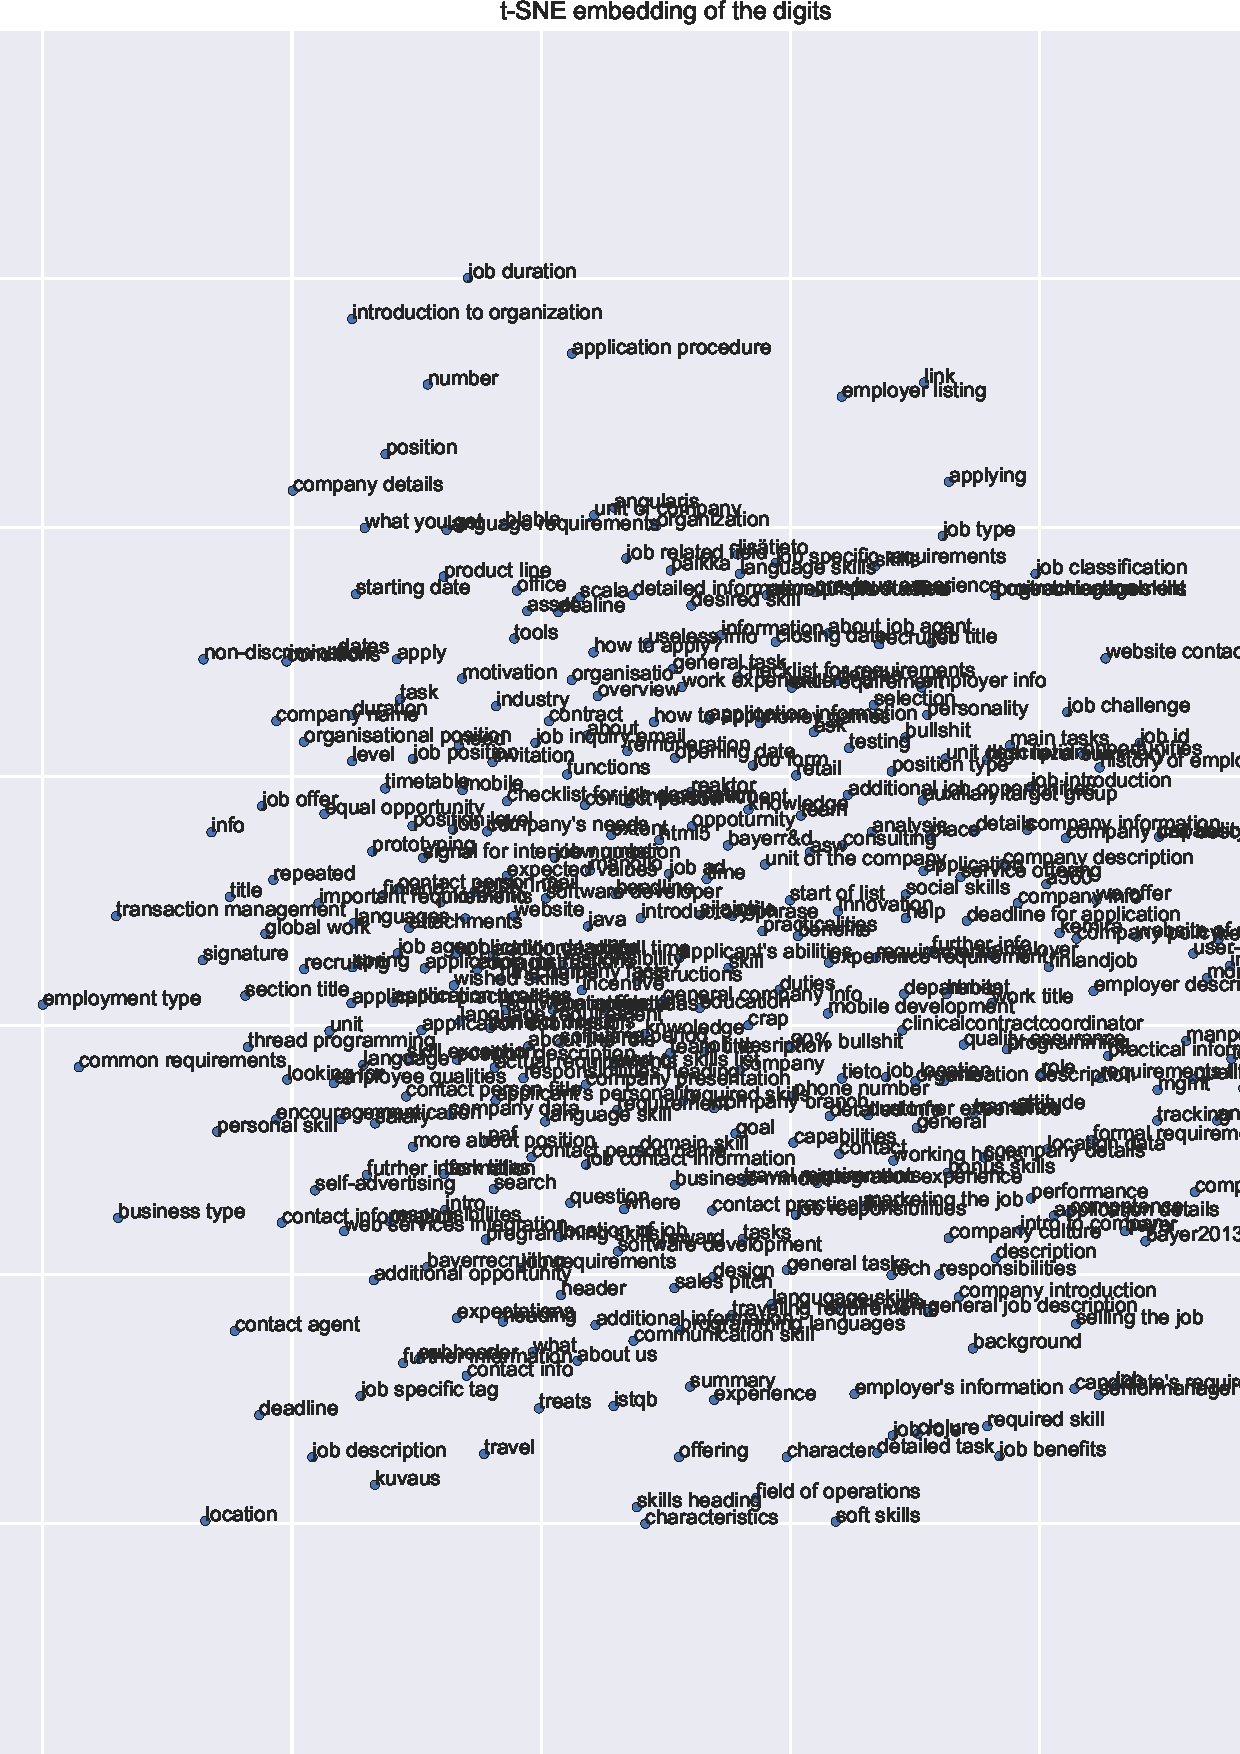
\includegraphics[width=\textwidth]{img/paragraph-data-tSNE.pdf}
    \caption{t-SNE Embedding}
\label{fig:paragraph-data-tSNE}
\end{figure}

\begin{figure}[h]
    \centering
    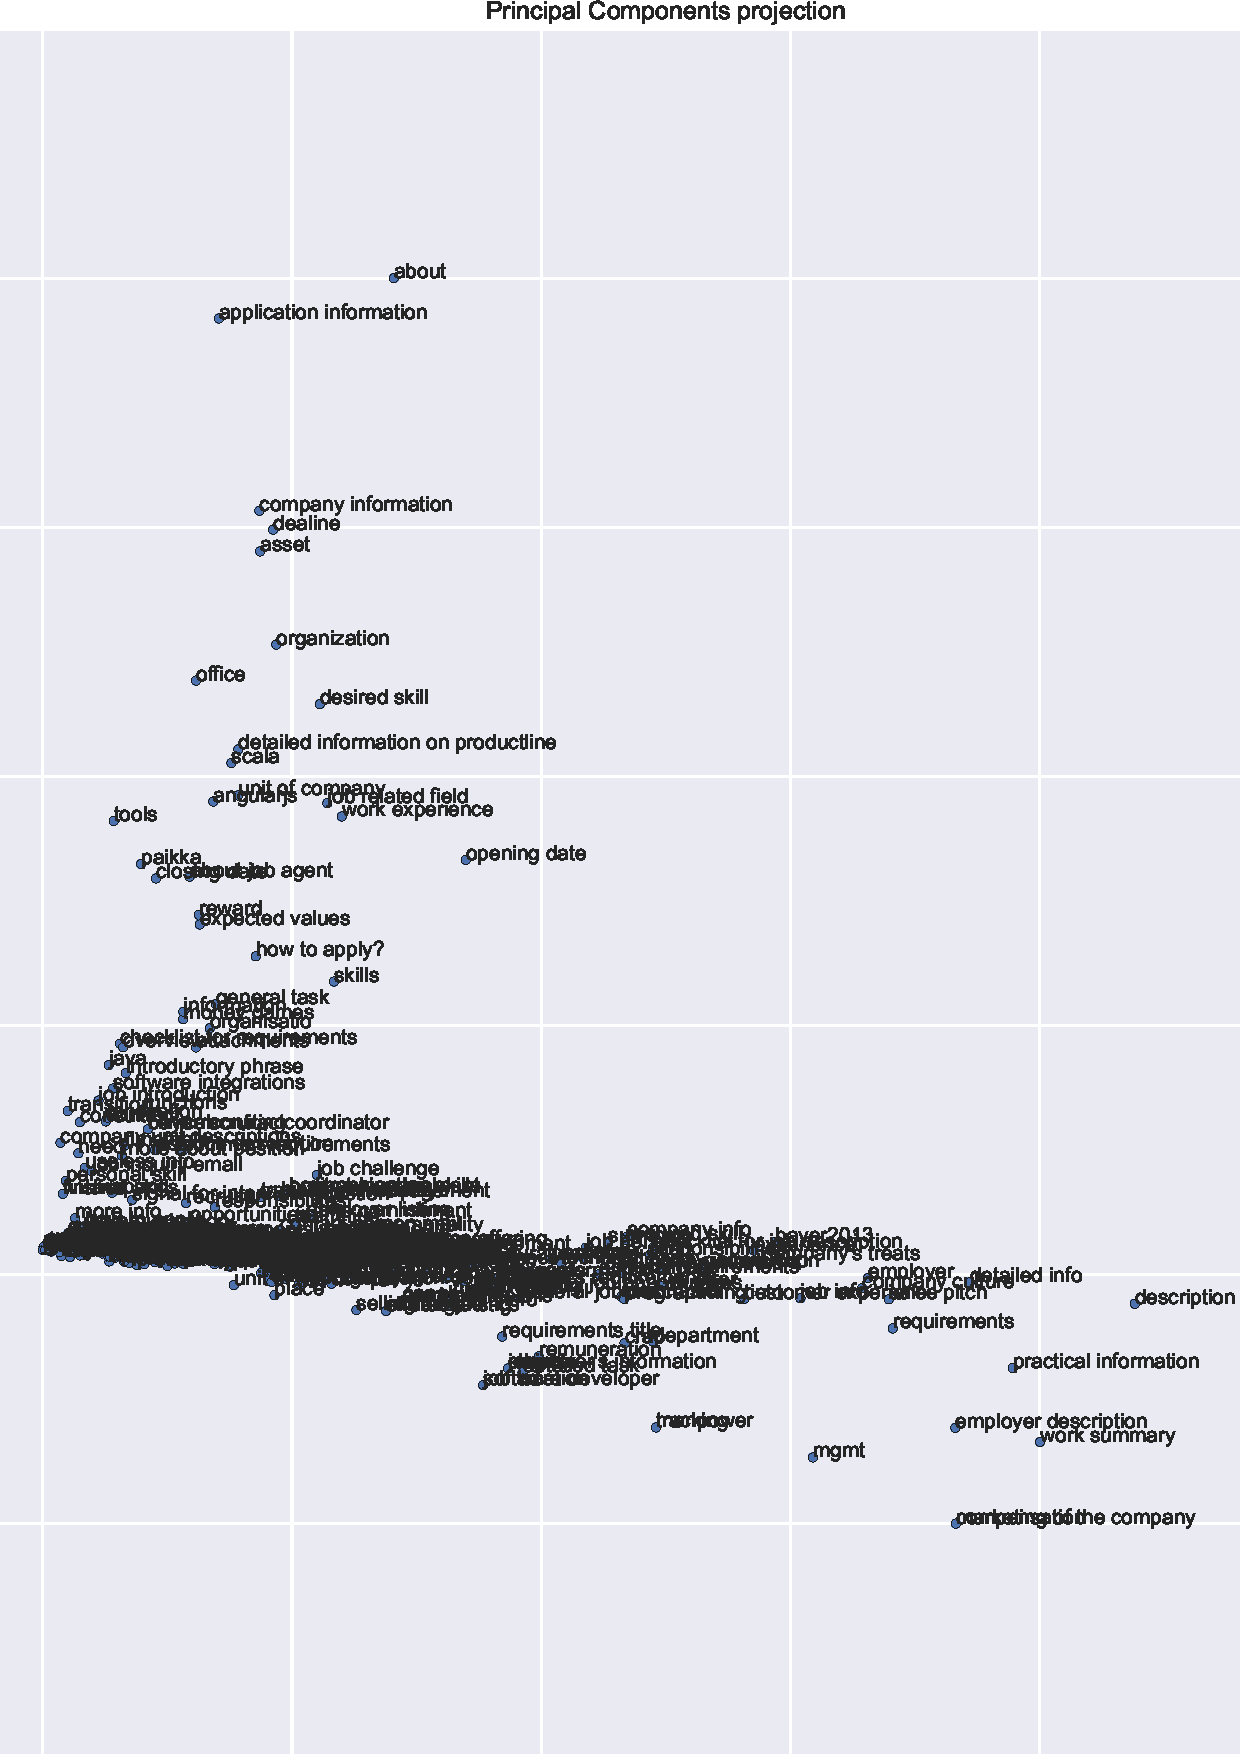
\includegraphics[width=\textwidth]{img/paragraph-data-principal-components-projection.pdf}
    \caption{Principal Components Projection}
\label{fig:paragraph-data-principal-components-projection}
\end{figure}

\todo{Comparison one-vs-rest and one-vs-one against linear machine}
\todo{Visualizations and embeddings of data in 2D (and decision boundaries?)}
\todo{show T-SNE embeddings of doc2vec vectors}


\subsection{Dataset 2}

\begin{figure}[h]
 % From http://localhost:8888/notebooks/thesis/experiments/vector-space-models/Vector%20Space%20Models.ipynb#Setup
    \centering
    \begin{subfigure}[b]{0.46\textwidth}
        \includegraphics[width=\textwidth]{img/sentence-data-judgement-confidence.pdf}
        \caption{Confidence}
\label{fig:sentence-data-judgement-confidence}
    \end{subfigure}
~%add desired spacing between images, e. g. ~, \quad, \qquad, \hfill etc.
    %(or a blank line to force the subfigure onto a new line)
    \begin{subfigure}[b]{0.43\textwidth}
        \includegraphics[width=\textwidth]{img/sentence-data-judgement-confidence-cumulative.pdf}
        \caption{Cumulative Confidence}
\label{fig:sentence-data-judgement-confidence-cumulative}
    \end{subfigure}
    \caption{Amount of label judgements versus label confidence of the sentence label data collected via crowdflower}
\label{fig:sentence-data-judgements}
\end{figure}



\begin{figure}[h]
  % From http://localhost:8888/notebooks/thesis/experiments/vector-space-models/Vector%20Space%20Models.ipynb#Setup
    \centering
    \includegraphics[width=\textwidth]{img/sentence-data-label-dist.pdf}
    \caption{Distribution of labels in sentence data}
\label{fig:sentence-data-label-dist}
\end{figure}

\section{Problem Definition: Text Classification}
\label{sec:Problem Definition: Text Classification}

% !TEX root = ../thesis.tex
% !TEX spellcheck = en-US

\clearpage

\section{Problem Definition}
\label{sec:Problem Definition}

This section will formally and mathematically define the research problem that was chosen as a focus for this thesis. First the more general problem known in the machine learning literature as \emph{Text Classification} is defined, then the research problem of this thesis termed \emph{Multi-class Sentence Classification} is formalized as a special case of text classification. Finally the dataset used as a basis to evaluate problem is described in detail.

\subsection{Context: Definition of Text Classification}
\label{subs:Context: Definition of Text Classification}

\begin{wrapfigure}{r}{0.5\textwidth}
  \begin{center}
    \includegraphics[width=0.5\textwidth]{img/bipartite-graph-text-classification}
  \end{center}
  \caption{Text classification visualized as a bipartite graph. Here the multi-label setting is shown where no additional constraints are enforced on the problem and hence each document can be assigned to multiple categories}
\label{fig:bipartite-graph-text-classification}
\end{wrapfigure}

Text classification, also known as text categorization, is the task of predicting a \emph{mapping} $\widetilde{\Phi} : \mathcal{D} \times \mathcal{C} \rightarrow \{True, False\}$ between a set of \emph{documents} $\mathcal{D}$ and a set of \emph{classes} or \emph{categories} $\mathcal{C}$ using a model function $\Phi : \mathcal{D} \times \mathcal{C} \rightarrow \{True, False \}$.
We thus aim to predict as well as possible the documents associated with each category or vice versa the categories that each document belongs into. The former is called \emph{category-pivoted} text classification whereas the latter is referred to as \emph{document-pivoted} text classification --- the setting that we shall focus on from here onwards.
The mapping $\widetilde{\Phi}$ can be represented as a bipartite graph between the set of documents $\mathcal{D}$ and the set of categories $\mathcal{C}$ as shown in Figure~\ref{fig:bipartite-graph-text-classification}. In this representation vertices in the graph represent a $True$ value in the mapping, indicating that the document and category are associated with each other, while missing vertices indicate that they are not which corresponds to a $False$ value in the mapping.

Categories $\mathcal{C}$ are given as symbolic labels and documents $\mathcal{D}$ as sequences of text with variable length. It is usually assumed that no additional information such as metadata or other \emph{exogenous knowledge} is available on neither labels nor documents.
As the survey on automatic text classification by~\cite{Sebastiani:2002aa} points, out a consequence of relying solely on \emph{endogenous knowledge}, especially the semantics of a text, is that there is no objective ground truth to this task in most settings since semantics are a \emph{subjective} notion: \textquote{This is exemplified by the phenomenon of inter-indexer inconsistency~\cite{Cleverdon:1984aa}: when two human experts decide whether to classify document $d_j$ under category $c_i$, they may disagree, and this in fact happens with relatively high frequency. A news article on Clinton attending Dizzy Gillespie’s funeral could be filed under Politics, or under Jazz, or under both, or even under neither, depending on the subjective judgment of the expert.}

Additional constraints can be imposed on the problem to adapt it for different application scenarios. Firstly text classification can be either framed as \emph{single-label} classification where each document is assigned to only one single category or \emph{multi-label} classification where an assignment to several categories or also no category is possible. The single-label case can be further separated into \emph{dichotomous} or \emph{binary} classification where the presence or absence of only a single class is predicted and \emph{multi-class} classification where one of multiple, mutually exclusive classes is predicted for each document.
Multi-class classification can thus be seen as multi-label classification with the additional constraint of classes being mutually exclusive.
If labels are assumed to be statistically independent multi-label classification can also be reformulated as $|\mathcal{C}|$ individual binary classification problems, potentially allowing much simpler modeling at the cost of introducing inductive bias through a strong assumption.

% In order to measure how successfully we are tackling the problem of text classification we need metrics that measure the effectiveness of our algorithm given a dataset. These will be discussed in Section~\ref{sub:Evaluation}.

\subsection{Problem Formalism: Multi-class Sentence Classification}
\label{subs:Problem Formalism: Multi-class Sentence Classification}

The prediction task in the scope of this thesis is \emph{Multi-class Sentence Classification} which shall be formulated as a special case of Text Classification defined above. Specifically the goal is to perform \emph{document-pivoted Multi-class Text Classification} where the documents $\mathcal{D}$ are the set of all sentences $S$ drawn \emph{uniformly and independently} at random from a set of job advertisements $\mathcal{J}$, and the classes $\mathcal{C}$ are set to be the following set of mutually exclusive labels $\mathcal{L} = \{ \text{benefits}, \text{candidate}, \text{company}, \text{job}, \text{nextsteps}, \text{other} \}$. We thus allow for no knowledge to be used regarding the origin of a sentence $s_i$, meaning that the prediction of each sentence is independent must assume the same prior information. The task can hence be expressed as predicting true label $l_i$ for a sentence $s_i$, i.e.\ finding the mapping $\widetilde{\Phi} : \mathcal{S} \rightarrow \mathcal{L}$.

\subsection{Dataset Used for Evaluation}
\label{subs:Dataset Used for Evaluation}

The performance of approaching the research problem will be evaluated using a dataset that was designed and created specifically for the purpose of this work. For detailed information on the process and design decisions involved please refer to Section~\ref{sub:Definition Phase: Framing the Problem} (\nameref{sub:Definition Phase: Framing the Problem}). Here the key characteristics of the data will be shown.

\begin{figure}[h]
  % From http://localhost:8888/notebooks/thesis/experiments/vector-space-models/Vector%20Space%20Models.ipynb#Setup
    \centering
    \includegraphics[width=\textwidth]{img/sentence-data-label-dist.pdf}
    \caption{Distribution of labels in sentence data}
\label{fig:sentence-data-label-dist}
\end{figure}

The data from this set stems from job advertisements created by companies using the \gls{Sanoma}'s service \gls{Oikotie Tyopaikat} in Finland. The dataset consists of 118780 job ads published between the September 01, 2012 and December 01, 2015. Each job posting contains many fields of associated metadata such as the title of the job posting, the time of creation and many more. Of these only the \emph{job description} was chosen as a basis for this task since --- as pointed out previously in Section~\ref{subs:Context: Definition of Text Classification} --- the task of interest was pure text classification without exogenous knowledge with the motivation to better understand unstructured data such as the job description which does not follow a specific format.

Using the tool \gls{langdetect} 9928 of these job ads were identified to be written in English language which is about 8.4\% as opposed 75\% of postings that are written in Finnish.
In order to form the sentence dataset 400 job english listings were then selected at random and converted into a set all 9948 sentences occurring in these listings using the \emph{Punkt Sentence Tokenizer}\footnote{See \url{http://www.nltk.org/api/nltk.tokenize.html\#module-nltk.tokenize.punkt}} of the \gls{NLTK}. Afterwards the sentences were converted from HTML into raw text using the \gls{Beautiful Soup} software package and labels were collected using the \gls{crowd sourcing} service \gls{CrowdFlower} as described in Section~\ref{subs:Multi-class Sentence Classification} using the fixed six labels from the problem definition above: \emph{benefits, candidate, company, job, nextsteps, other}. Each label with a description that was given when collecting the data and an example sentence can be seen in Table~\ref{tab:Labels, Description, Example Sentences}.

\begin{table}[h]
  \begin{center}
  \begin{tabularx}{\textwidth}{l | X | X}
    \toprule
    Label & Description & Example Sentence \\
    \midrule
    benefits & \textbf{Benefits}: Rewards, opportunities, reasons to apply, \ldots & And we like to think we’ll give you an enjoyable and inspiring place to spend your working day. \\
    candidate & \textbf{Candidate requirements}: Requirements, skills, experience, education, personality, \ldots & To succeed in this position it is essential to have strong experience of at least 5 years in international business development and/or international B2B sales and marketing. \\
    company & \textbf{Company information}: Company name, story, mission, structure, market share, \ldots & Progman is software house specialising in the development of software for Building Services. \\
    job & \textbf{Job description}: Role, responsibilities, location of work, type of employment, \ldots & Your main objective is to maximize Core Fleet, Dealer B2B, municipality and governmental orders and sales for PC and LCV range to local Fleets and businesses within defined geographical area. \\
    nextsteps & \textbf{Next steps}: Call to action, application procedure, contact, further information, \ldots & 040 75 67 316, Mon-Fri 10-14, or peas@temp-team.fi. \\
    other & \textbf{Other}: Does not fit into the above categories & URS’ \\
    \bottomrule
  \end{tabularx}
  \caption{Labels used for the task with their description that was given for the participants labelling the data and a sentence example for each label.}
\label{tab:Labels, Description, Example Sentences}
\end{center}
\end{table}

The resulting distribution of the labels is strongly skewed towards higher prevalence of several labels as shown in Figure~\ref{fig:sentence-data-label-dist}. For this reason the use of an unbiased evaluation metric was especially important and Matthews Correlation Coefficient met this criterion and was thus chosen (see Section~\ref{sub:Evaluation of Text Classification Methods} for more information on the chosen evaluation methods).

\include{./tex/approaches(background)}
% !TEX root = ../thesis.tex
% !TEX spellcheck = en-US

%% Leave first page empty
\thispagestyle{empty}

\section{Experiments}
\label{sec:Experiments}

\todo{Doc2Vec model is evaluated in 2 ways (normal and trained on inferred vectors)}

With the final problem definition and dataset in place experiments were set up to evaluate the performance of the different methods to approach this problem that that are explained in Section~\ref{sec:Methods}. In this section the research objectives of these experiments will be defined and the metrics used will be described. Afterwards the experimental setup for each of the methods in the same order as the results for each approach will be presented in Section~\ref{sec:Results}.

\subsection{Objectives and Metrics}
\label{sub:Objectives and Metrics}

The experiments had simple objectives: The goal was to evaluate each method in terms of its effectiveness using a prediction metric well-suited for this problem. Further additional considerations, especially algorithmic time and space complexity were taken into account by comparing methods with regards to their runtime and need for computational resources.

\glsreset{MCC}

As a metric for predictive performance \gls{MCC} was chosen. This metric is used relatively rarely used as opposed to e.g.\ the F1 score that is common in the \gls{IR} literature where ignoring True Negatives can be tolerated. As an example we do not generally care if a search engine predicts correctly all the billions of website we don't want to see for a search query as long as it retrieves enough relevant ones.
With the dataset at hand though the needs were different and a metric was needed that can reliably and without bias measure prediction despite a strongly skewed distribution of labels, and stratified sampling to achieve a balanced distribution was not an option since the dataset was too small. \gls{MCC} fulfills these criteria as Section~\ref{sub:Evaluation Metrics for Text Classification} points out and additionally is easy to interpret as it is a correlation score between 1 (absolute correlation) and -1 (absolute anti-correlation) as opposed to e.g.\ the categorical cross-entropy error. In some experiments additionally further metrics were measured.

\subsection{Baseline}
\label{par:Baseline}

As a baseline for comparing the performance of classification two different guessing strategies were used, namely uniform and stratified guessing.
Uniform guessing refers to a predictor that samples from the given classes assuming a uniform distribution whereas stratified guessing takes the label distribution in the data as the underlying probability distribution.
Then both methods just sample from these distributions to produce ``predictions'', while ignoring the actual input data.

\todo{mention score for baselines being 0 for MCC}

\subsection{Text Classification Using Vector Space Models}
\label{sub:Text Classification Using Vector Space Models}

A popular way to approach text classification and other tasks in natural language processing is to build a model that maps data into a vector space so that distance between data points in this space translates to similarity between the objects (see Section~\ref{sub:Vector Space Models}). The resulting vector representation of the data can then be fed into various learning algorithms. This section describes the experiments performed to study this approach to the sentence classification problem as defined in Section~\ref{subs:Problem Formalism: Multi-class Sentence Classification}.

First the different approaches to produce such vector representations are compared. Several methods were used to generate vectors from the data while limiting dimensionality to 300 --- a heuristically chosen value as performance for the models did not increase significantly after beyond it. These vectors were then compared in terms of performance using them as input to the very simple classification method Logistic Regression.

Second, the most well-performing candidates to produce vector representations were chosen and a set of more advanced classification techniques was applied to them.

\todo{baseline comparison missing in later experiments?}

\subsubsection*{Evaluation of Vector Space Models}
\label{subs:Evaluation of Vector Space Models}

\paragraph{N-gram Models}
\label{par:N-gram Models}

The first class of language models that was investigated for the task of multi-class classification are N-gram models that were explained in Section~\ref{subs:n-gram-language-models}. As mentioned, in essence this type of model relies on simple statistics which makes for straightforward computation but at the same time comes at cost of expressiveness, especially in terms of temporal dependencies between words.

As N-grams models come in a variety of variants the most important ones were used as hyper-parameters to the model and a grid search was carried out over a wide range of combinations over these. The specific hyper-parameter settings are listed in Table~\ref{tab:ngram-parameters}. The grid search was optimized with regards to \emph{Matthews Correlation Coefficient} (see Section~\ref{par:Matthews Correlation Coefficient for K classes}) using 5-fold cross-validated with three standard classifiers: Logistic Regression and Naive Bayes and SVM.

\paragraph{Bag-of-Means: An Averaged Word2Vec Model}
\label{par:Bag-of-Means: An Averaged Word2Vec Model}

Next a Bag-of-Means model as described in Section~\ref{subp:Bag-of-Means} was evaluated with the same set of classifiers. The model was evaluated on the same test and training data split as used for the N-gram model above. As a basis the pre-trained word-vectors from the Google News dataset\footnote{The dataset contains contains 300-dimensional vectors for 3 million words and phrases. The phrases were obtained using a simple data-driven approach described in~\cite{Mikolov:2013ab}. The dataset can be obtained on the following website: \url{https://code.google.com/archive/p/word2vec/}} were used and then for each document all word vectors were average to obtain the document vector.

\paragraph{Paragraph Vectors using Distributed Representations}
\label{par:Paragraph Vectors using Distributed Representations}

Next a vector space model was build using the approach proposed by~\cite{Le:2014aa} and described in more detail in Section~\ref{par:Distributed representations for documents}. Again there are several hyper-parameters to this model that are described in Section~\ref{subs:Language Models using Distributed Representations} and turn out to have a huge influence on its performance as the results below indicate. As this model is computationally quite expensive a grid search as for the N-gram model above was infeasible. Thus the effect of the hyper-parameters was studied by just varying them one at a time while keeping the others fixed, using a Logistic Regression classifier with 5-fold cross-validation.

\subsubsection*{Evaluation of Classification Methods}
\label{subs:Evaluation of Classification Methods}

\paragraph{Logistic Regression}
\label{par:Logistic Regression}

\paragraph{Decision Tree}
\label{par:Decision Tree}

\paragraph{Naive Bayes}
\label{par:Naive Bayes}

\paragraph{Support Vector Machine}
\label{par:Support Vector Machine}

\paragraph{$k$ Nearest Neighbors}
\label{par:k Nearest Neighbors}

\paragraph{Random Forest}
\label{par:Random Forest}

\paragraph{Vanilla Neural Network}
\label{par:Vanilla Neural Network}

\paragraph{Deep Neural Network}
\label{par:Deep Neural Network}

\paragraph{Convolutional Neural Network}
\label{par:Convolutional Neural Network}



\subsection{Sequential Text Classification}

% !TEX root = ../thesis.tex
% !TEX spellcheck = en-US

% doc2vec: highest value is highlighted

% How did I approach the problem, what methods did I evaluate

\clearpage

\section{Results}
\label{sec:Results}

\subsection{Baseline}
\label{sub:Baseline}

Both, uniform and stratified guessing achieve a Matthews Correlation Coefficient score of around 0 (averaged over 1000 runs) as expected for guessing strategies (see Section~\ref{subs:informedness-markedness-mcc}). On the other hand the accuracy for uniform guessing is around 0.16 which corresponds to $1/\text{K}$ for the K classes and around 0.26 for stratified guessing which reflects the skew of the label distribution.
Figure~\ref{fig:guessing-conf-matrix} shows the confusion matrices for these baseline variants in absolute and normalized form, revealing the properties of these guessing strategies.

\begin{figure}[h]
 % From http://localhost:8888/notebooks/thesis/experiments/vector-space-models/Vector%20Space%20Models.ipynb#Baseline:-Guessing-Strategies
    \centering
    \begin{subfigure}[b]{0.47\textwidth}
        \includegraphics[width=\textwidth]{img/exp-vector-space/guessing-conf-matrix-uniform.pdf}
        \caption{Uniform, absolute}
\label{fig:guessing-conf-matrix-uniform}
    \end{subfigure}
~%add desired spacing between images, e. g. ~, \quad, \qquad, \hfill etc.
    %(or a blank line to force the subfigure onto a new line)
    \begin{subfigure}[b]{0.48\textwidth}
        \includegraphics[width=\textwidth]{img/exp-vector-space/guessing-conf-matrix-uniform-normalized.pdf}
        \caption{Uniform, normalized}
\label{fig:guessing-conf-matrix-uniform-normalized}
    \end{subfigure}
~
    \begin{subfigure}[b]{0.47\textwidth}
        \includegraphics[width=\textwidth]{img/exp-vector-space/guessing-conf-matrix-stratified.pdf}
        \caption{Stratified, absolute}
\label{fig:guessing-conf-matrix-stratified}
    \end{subfigure}
~
    %add desired spacing between images, e. g. ~, \quad, \qquad, \hfill etc.
    %(or a blank line to force the subfigure onto a new line)
    \begin{subfigure}[b]{0.48\textwidth}
        \includegraphics[width=\textwidth]{img/exp-vector-space/guessing-conf-matrix-stratified-normalized.pdf}
        \caption{Stratified, normalized}
\label{fig:guessing-stratified-normalized}
    \end{subfigure}
    \caption{Confusion matrices of uniform and stratified guessing strategies. }
\label{fig:guessing-conf-matrix}
\end{figure}

\subsection{Text Classification Using Vector Space Models}
\label{sub:Text Classification Using Vector Space Models}

\subsubsection{N-gram Models}

\todo{intro here}

\begin{table}[h]
  \begin{center}
  \begin{tabular}{ l l l}
    \toprule
    Hyper-Parameter & N-gram Type: Words & N-gram Type: Characters \\
    \midrule
    N-gram Range (Range) & [1,1], [1,2], [1,3], [2,3], [3,3] & [1,5], [1,10], [5,10], [5,15] \\
    Stop Words & English, None & N/A \\
    Vector Size (Size) & 10, 100, 300 & 10, 100, 300 \\
    IDF & Yes, No & Yes, No \\
    Norm & L1, L2, None & L1, L2, None \\
    Sub-linear TF & Yes, No & Yes, No \\
    \bottomrule
  \end{tabular}
  \caption{Parameter search space word and character level N-gram models}
\label{tab:Ngram Parameters}
\end{center}
\end{table}

The 5 best results of these exhaustive grid searches can be seen in Table~\ref{tab:Ngram Grid Search} below.

\begin{table}[h]
  \begin{center}
  \begin{tabular}{ l l l l l l l l }
    \toprule
    Type & Range & Stop words & Size & IDF & Norm & Sub-linear TF & MCC Score \\
    \midrule
    Word & [1,1] & None & 300 & Yes &  & Yes & 0.689 \\
    Word & [1,1] & None & 300 & Yes &  & No & 0.687 \\
    Word & [1,1] & None & 300 & No &  & Yes & 0.682 \\
    Word & [1,1] & None & 300 & No &  & No & 0.682 \\
    Word & [1,1] & None & 300 & Yes & L2 & Yes & 0.68 \\
    % Word & [1,1] & None & 300 & Yes & L2 & No & 0.678 \\
    % Word & [1,2] & None & 300 & No &  & Yes & 0.677 \\
    % Word & [1,2] & None & 300 & Yes & L2 & Yes & 0.676 \\
    % Word & [1,2] & None & 300 & Yes & L2 & No & 0.675 \\
    % Word & [1,2] & None & 300 & No &  & No & 0.675 \\
    \midrule
    Word & [1,1] & None & 300 & No & & Yes & 0.659  \\
    Word & [1,1] & None & 300 & No & & No & 0.656 \\
    Word & [1,2] & None & 300 & No & & Yes & 0.655 \\
    Word & [1,2] & None & 300 & No & & No & 0.655 \\
    Word & [1,3] & None & 300 & No & & No & 0.65 \\
    % Word & [1,1] & None & 300 & Yes & L2 & Yes & 0.648 \\
    % Word & [1,1] & None & 300 & Yes & L2 & No & 0.648 \\
    % Word & [1,3] & None & 300 & No & & Yes & 0.648 \\
    % Word & [1,2] & None & 300 & Yes & L2 & No & 0.647 \\
    % Word & [1,2] & None & 300 & Yes & L2 & Yes & 0.646 \\
    \midrule
    Word & [1,1] & None & 300 & Yes & & Yes & 0.689 \\
    Word & [1,1] & None & 300 & Yes & & No  & 0.689 \\
    Word & [1,2] & None & 300 & Yes & & Yes & 0.677 \\
    Word & [1,2] & None & 300 & Yes & & No  & 0.677 \\
    Word & [1,3] & None & 300 & Yes & & Yes & 0.674 \\
    % Word & [1,3] & None    & 300 & Yes & & No  & 0.673 \\
    % Word & [1,1] & English & 300 & Yes & & Yes & 0.65 \\
    % Word & [1,1] & English & 300 & Yes & & No  & 0.65 \\
    % Word & [1,2] & English & 300 & Yes & & No  & 0.649 \\
    % Word & [1,2] & English & 300 & Yes & & Yes & 0.648 \\
    \bottomrule
  \end{tabular}
  \caption{Top 5 results of grid search over hyper-parameter space as listed in Table~\ref{tab:Ngram Parameters} using 5-fold cross-validated Logistic Regression (top), Naive Bayes (middle) and SVM (bottom) classifiers.}
\label{tab:Ngram Grid Search}
\end{center}
\end{table}

\todo{Why are the grid scores lower than the latter scores on the train/test split? Because they're averaged and only on the training data?}

Across all classifiers the following results on the hyper-parameters can be observed:

\paragraph{Type}
\label{par:Type}
Words as the atomic unit for N-grams consistently lead to better results. This is understandable as the search space of combinations of characters is significantly larger than the search space of known words.

\paragraph{Range}
\label{par:Range}
There are slight differences to be observed between the three classifiers used, but with all three models the best performance is achieved using Unigrams. Also all of the top results across all classifiers include Unigrams in the model while extending the range towards bigrams or trigrams.

\paragraph{Stop Words}
\label{par:Stop Words}
None of the top results of the performed grid searches used stop words. This is interesting as using stop-words to remove hand-picked, highly frequent words that do not carry much meaning is common practice. It seems there is information carried within these stop words. Of course this outcome is also influenced by the particular stop-list used (see Section~\ref{subp:Stop words}).

\paragraph{Size (matters)}
\label{par:Size}
For the searched settings the largest vector dimensionality of 300 achieves the best performance. This is not surprising as higher-dimensional vectors can capture more information about N-gram occurrences. However in practice the vector size must be limited as it grows with the vocabulary --- potentially at an exponential rate if N-grams other than Unigrams are used. Also very high dimensionality often leads to decreased performance in terms of generalization of the model.

\paragraph{IDF}
\label{par:IDF}
There is no consensus between the classifiers on whether or not to weigh the N-gram frequencies by the \emph{inverse document frequency} (see Section~\ref{subp:TF.IDF weighting}). Thus it seems advisable to lead this parameter free for and evaluate both variants with a given classifier. For logistic regression however the performance differences are marginal and so the choice for this parameter seems somewhat arbitrary.

\paragraph{Norm}
\label{par:Norm}
Is seems that normalizing the vectors in most cases does not lead to any performance gains. Again this is an often recommended practice but here it does not seem to add any value to the model.


\paragraph{Sub-linear TF}
\label{par:Sub-linear TF}
Applying sub-linear TF (see Section~\ref{subp:Sublinear TF scaling}) does not seem to affect the results much and the choice of this parameter can hence be chosen almost arbitrarily as well, although here for all three classifiers applying it leads to a marginal improvement.

Table~\ref{tab:Ngram Grid Search Scores} shows the scores of each classifier using the best N-gram model. It is evident that here logistic regression actually performs best as it offers both, a good accuracy as well as the highest score for Matthews Correlation Coefficient.

\begin{table}[h]
  \begin{center}
  \begin{tabular}{ r | *2l | *2l }
    \toprule
     & \multicolumn{2}{c|}{Training} & \multicolumn{2}{|c}{Validation}\\
    Classifier & Accuracy & MCC & Accuracy & MCC \\
    \midrule
    Logistic Regression & 0.824 & 0.761 & 0.787 & 0.708 \\
    Naive Bayes         & 0.769 & 0.681 & 0.767 & 0.677 \\
    SVM                 & 0.835 & 0.681 & 0.786 & 0.700 \\
    \bottomrule
  \end{tabular}
  \caption{Performance of each best N-gram model with Logistic Regression and Naive Bayes on the validation data}
\label{tab:Ngram Grid Search Scores}
\end{center}
\end{table}

\begin{figure}[h]
    \centering
    \begin{subfigure}[b]{0.32\textwidth}
        \includegraphics[width=\textwidth]{img/exp-vector-space/ngram-conf-matrix-logreg-normalized.pdf}
        \caption{Logistic Regression}
\label{fig:ngram-conf-matrix-logreg-normalized}
    \end{subfigure}
    \begin{subfigure}[b]{0.32\textwidth}
        \includegraphics[width=\textwidth]{img/exp-vector-space/ngram-conf-matrix-naivebayes-normalized.pdf}
        \caption{Naive Bayes}
\label{fig:ngram-conf-matrix-naivebayes-normalized}
    \end{subfigure}
    \begin{subfigure}[b]{0.32\textwidth}
        \includegraphics[width=\textwidth]{img/exp-vector-space/ngram-conf-matrix-svm-normalized.pdf}
        \caption{SVM}
\label{fig:ngram-conf-matrix-svm-normalized}
    \end{subfigure}
    \caption{Normalized confusion matrices all three classifiers using the best N-gram model found via cross-validated grid search. Both Naive Bayes as well as SVM show label bias towards the prevalent class \emph{candidate}.}
\label{fig:ngram-conf-matrix}
\end{figure}
\todo{properly align visualization}

Figure~\ref{fig:ngram} shows projections of the of the constructed feature space using the best model that was optimized with Logistic Regression. This visualization shows the separability of the classes in this space. Especially the PCA projection here reveals that it is clearly possible to separate the classes until a certain point.

\begin{figure}[h]
    \centering
    \begin{subfigure}[b]{0.48\textwidth}
      \includegraphics[width=\textwidth]{img/exp-vector-space/ngram-pca.pdf}
      \caption{PCA projection}
\label{fig:ngram-pca}
    \end{subfigure}
~
    %add desired spacing between images, e. g. ~, \quad, \qquad, \hfill etc.
    %(or a blank line to force the subfigure onto a new line)
    \begin{subfigure}[b]{0.48\textwidth}
      \includegraphics[width=\textwidth]{img/exp-vector-space/ngram-tsne.pdf}
      \caption{t-SNE projection}
\label{fig:ngram-tsne}
    \end{subfigure}
    \caption{Document vectors produced by the best N-gram model (optimized w.r.t. Logistic Regression) projected onto the first 2 principal components (left) and project using t-SNE projection.}
\label{fig:ngram}
\end{figure}

\subsubsection{Bag-of-Means Model}

 The results can be seen in Table~\ref{tab:Bag-Of-Means Results}.

\begin{table}[h]
  \begin{center}
  \begin{tabular}{ r | *2l | *2l }
    \toprule
     & \multicolumn{2}{c|}{Training} & \multicolumn{2}{|c}{Validation}\\
    Classifier & Accuracy & MCC & Accuracy & MCC \\
    \midrule
    Logistic Regression & 0.797 & 0.722 & 0.784 & 0.702 \\
    Naive Bayes         & 0.337 & 0.271 & 0.320 & 0.251 \\
    SVM                 & 0.545 & 0.356 & 0.562 & 0.379 \\
    \bottomrule
  \end{tabular}
  \caption{Performance base classifiers using the Bag-of-Means model}
\label{tab:Bag-Of-Means Results}
\end{center}
\end{table}

The model performs well using Logistic Regression and is almost on par with the best N-gram model. This is surprising as performance previously reported to be rather poor as mention in Section~\ref{subp:Bag-of-Means}. On the other hand the variance in results between the classifiers is huge and especially Naive Bayes seems to perform extremely poor. Further investigation into the use of different classifiers could shed light into these diverging results which are not observed using the N-gram models in the section above. The confusion matrices in Figure~\ref{fig:bom-conf-matrix} reveal strong label bias in the case of Naive Bayes and SVM, although it is unclear where this stems from. Figure~\ref{fig:bom} makes clear though that there is a somewhat meaningful mapping into the feature space. \todo{mention one-vs-all scheme for log reg? also for ngrams above}

\begin{figure}[h]
    \centering
    \begin{subfigure}[b]{0.32\textwidth}
        \includegraphics[width=\textwidth]{img/exp-vector-space/bom-conf-matrix-logreg-normalized.pdf}
        \caption{Logistic Regression}
\label{fig:bom-conf-matrix-logreg-normalized}
    \end{subfigure}
    \begin{subfigure}[b]{0.32\textwidth}
        \includegraphics[width=\textwidth]{img/exp-vector-space/bom-conf-matrix-naivebayes-normalized.pdf}
        \caption{Naive Bayes}
\label{fig:bom-conf-matrix-naivebayes-normalized}
    \end{subfigure}
    \begin{subfigure}[b]{0.32\textwidth}
        \includegraphics[width=\textwidth]{img/exp-vector-space/bom-conf-matrix-svm-normalized.pdf}
        \caption{SVM}
\label{fig:bom-conf-matrix-svm-normalized}
    \end{subfigure}
    \caption{Normalized confusion matrices of all three classifiers using the Bag-of-Means model.}
\label{fig:bom-conf-matrix}
\end{figure}

\begin{figure}[h]
    \centering
    \begin{subfigure}[b]{0.48\textwidth}
      \includegraphics[width=\textwidth]{img/exp-vector-space/bom-pca.pdf}
      \caption{PCA projection}
\label{fig:bom-pca}
    \end{subfigure}
~
    %add desired spacing between images, e. g. ~, \quad, \qquad, \hfill etc.
    %(or a blank line to force the subfigure onto a new line)
    \begin{subfigure}[b]{0.48\textwidth}
      \includegraphics[width=\textwidth]{img/exp-vector-space/bom-tsne.pdf}
      \caption{t-SNE projection}
\label{fig:bom-tsne}
    \end{subfigure}
    \caption{Document vectors produced by Bag-of-Means model (optimized w.r.t. Logistic Regression) projected onto the first 2 principal components (left) and projected using t-SNE projection. It is clear that even though the vectors are simply obtained by averaging they do indeed produce somewhat seperable manifolds.}
\label{fig:bom}
\end{figure}

\subsubsection{Paragraph Vectors using Distributed Representations}


The next sections will briefly outline the results of these tests:\footnote{All tables in this section will use the following abbreviations: \emph{type}: Model Type, i.e. PV-DM vs. PV-DBOW; \emph{size}: Vector Size; \emph{window}: Window Size; \emph{negative}: Negative Sampling value $k$; \emph{hs}: Hierarchical Softmax used; \emph{sample}: Frequent word sub-sampling threshold; \emph{MCC}: Matthews Correlation Coefficient}

\paragraph{Vector Size}
As was to expect the vector size of the model correlates with the performance. Again the highest chosen dimensionality was 300 which yielded the best results with a Matthews Correlation Coefficient of 0.53, however the difference to a 100-dimensional model was marginal with 1\% absolute improvement. Surprisingly even a 10-dimensional vector space model is capable of achieving almost best results with a difference of only 2\% to the 300-dimensional model. Even a 2-dimensional model could achieve a MCC score of 14\%.

\begin{table}[h]
  \begin{center}
    \begin{tabular}{ c | *2c | *2c }
      \toprule
       & \multicolumn{2}{c|}{MCC Training} & \multicolumn{2}{|c}{MCC Test}\\
      Vector Size & Trained & Inferred & Trained & Inferred \\
      \midrule
      2   & 0.302 & 0.255 & 0.173 & 0.251 \\
      10  & 0.457 & 0.417 & 0.296 & \textbf{0.405} \\
      100 & 0.535 & 0.358 & 0.341 & 0.384 \\
      300 & 0.575 & 0.363 & 0.347 & 0.393 \\
      \bottomrule
    \end{tabular}
  \caption{Matthews Correlation Coefficient with varying vector size.}
\label{tab:Paragraph Vector Parameter Results Size}
\end{center}
\end{table}

\begin{figure}[h!]
    \centering
    \begin{subfigure}[b]{0.49\textwidth}
      \includegraphics[width=\textwidth]{img/exp-vector-space/doc2vec_vector_size_2}
      \caption{Vector Size: 2}
\label{fig:doc2vec_vector_size_2}
    \end{subfigure}
    \begin{subfigure}[b]{0.49\textwidth}
      \includegraphics[width=\textwidth]{img/exp-vector-space/doc2vec_vector_size_10}
      \caption{Vector Size: 10}
\label{fig:doc2vec_vector_size_10}
    \end{subfigure}
    \begin{subfigure}[b]{0.49\textwidth}
      \includegraphics[width=\textwidth]{img/exp-vector-space/doc2vec_vector_size_100}
      \caption{Vector Size: 100}
\label{fig:doc2vec_vector_size_100}
  \end{subfigure}
  \begin{subfigure}[b]{0.49\textwidth}
    \includegraphics[width=\textwidth]{img/exp-vector-space/doc2vec_vector_size_300}
    \caption{Vector Size: 300}
\label{fig:doc2vec_vector_size_300}
  \end{subfigure}
\caption{test}
\label{fig:doc2vec_vector_size}
\end{figure}

\paragraph{Frequent Word Sub-Sampling}
Frequent word sub-sampling can boost performance quite much, but again choosing the right value for this hyper-parameter is key. The training behavior with different sampling thresholds differs quite much. Figure~\ref{fig:doc2vec-param-sample} shows the training with different values with 100 passes over the dataset. A good value seems to be $10^{-5}$ which achieves an MCC score of 0.697 and is on-par with the best N-gram model. Interestingly not using sub-sampling in this setup seemed to be overfitting as the score decreases quite drastically with more training passes. A similar effect is observed with a higher threshold of $10^{-4}$ but much less strong. Choosing a lower threshold of $10^{-6}$ leads to very poor performance with an MCC score of only 0.07.

\begin{table}[h]
  \begin{center}
    \begin{tabular}{ c | *2c | *2c }
      \toprule
       & \multicolumn{2}{c|}{MCC Training} & \multicolumn{2}{|c}{MCC Test}\\
      Sub-sampling threshold & Trained & Inferred & Trained & Inferred \\
      \midrule
      No sub-sampling & 0.536 & 0.363 & 0.336 & 0.384 \\
      1e-4 & 0.627 & 0.377 & 0.315 & \textbf{0.397} \\
      1e-5 & 0.599 & 0.250 & 0.173 & 0.247 \\
      1e-6 & 0.431 & 0.147 & 0.106 & 0.129 \\
    \bottomrule
  \end{tabular}
  \caption{Matthews Correlation Coefficient with varying frequent word sub-sampling threshold.}
\label{tab:Paragraph Vector Parameter Results Sample}
\end{center}
\end{table}

\begin{figure}[h!]
    \centering
    \begin{subfigure}[b]{0.49\textwidth}
      \includegraphics[width=\textwidth]{img/exp-vector-space/doc2vec_sample_0}
      \caption{No Sub-Sampling}
\label{fig:doc2vec_sample_0}
    \end{subfigure}
    \begin{subfigure}[b]{0.49\textwidth}
      \includegraphics[width=\textwidth]{img/exp-vector-space/doc2vec_sample_1e-4}
    \caption{Sub-Sampling Threshold: 1e-4}
\label{fig:doc2vec_vector_size_1e-4}
    \end{subfigure}
    \begin{subfigure}[b]{0.49\textwidth}
      \includegraphics[width=\textwidth]{img/exp-vector-space/doc2vec_sample_1e-5}
      \caption{Sub-Sampling Threshold: 1e-5}
\label{fig:doc2vec_vector_size_1e-5}
  \end{subfigure}
  \begin{subfigure}[b]{0.49\textwidth}
    \includegraphics[width=\textwidth]{img/exp-vector-space/doc2vec_sample_1e-6}
    \caption{Sub-Sampling Threshold: 1e-6}
\label{fig:doc2vec_sample_1e-6}
  \end{subfigure}
\caption{test}
\label{fig:doc2vec_sample}
\end{figure}

\paragraph{Hierarchical Softmax}
Using hierarchical softmax increased the performance, leading to a 12\% absolute difference in terms of MCC score. This result is counter-intuitive as using the hierarchical softmax should as an approximation be less performant. However it might simply mitigate overfitting of the model.

\begin{table}[h]
  \begin{center}
    \begin{tabular}{ c | *2c | *2c }
      \toprule
       & \multicolumn{2}{c|}{MCC Training} & \multicolumn{2}{|c}{MCC Test}\\
      Hierarchical Softmax & Trained & Inferred & Trained & Inferred \\
      \midrule
      Not used & 0.364 & 0.195 & 0.201 & 0.236 \\
      Used     & 0.534 & 0.365 & 0.340 & \textbf{0.387} \\
    \bottomrule
  \end{tabular}
  \caption{Matthews Correlation Coefficient with and without using hierarchical softmax.}
\label{tab:Paragraph Vector Parameter Results Hierarchical Softmax}
\end{center}
\end{table}

\begin{figure}[h!]
    \centering
    \begin{subfigure}[b]{0.49\textwidth}
      \includegraphics[width=\textwidth]{img/exp-vector-space/doc2vec_hs_0}
      \caption{Without Hierarchical Softmax}
\label{fig:doc2vec_hs_0}
    \end{subfigure}
    \begin{subfigure}[b]{0.49\textwidth}
      \includegraphics[width=\textwidth]{img/exp-vector-space/doc2vec_hs_1}
    \caption{With Hierarchical Softmax}
\label{fig:doc2vec_hs_1}
    \end{subfigure}
\caption{test}
\label{fig:doc2vec_hs}
\end{figure}

\paragraph{Negative Sampling}
Negative Sampling generally increased the performance of the model and smaller values actually worked best out of the tested settings from 0 to 6. Choosing the number of negative samples to be 2 resulted in the best performance, but the absolute difference in performance was only about 6\% of achieved MMC score.

\begin{table}[h]
  \begin{center}
    \begin{tabular}{ c | *2c | *2c }
      \toprule
       & \multicolumn{2}{c|}{MCC Training} & \multicolumn{2}{|c}{MCC Test}\\
      Negative Sampling Value & Trained & Inferred & Trained & Inferred \\
      \midrule
      0 & 0.581 & 0.221 & 0.332 & 0.343 \\
      2 & 0.555 & 0.338 & 0.363 & \textbf{0.399} \\
      4 & 0.517 & 0.336 & 0.350 & 0.378 \\
      6 & 0.489 & 0.317 & 0.338 & 0.363 \\
    \bottomrule
  \end{tabular}
  \caption{Matthews Correlation Coefficient with varying negative sampling value.}
\label{tab:Paragraph Vector Parameter Results Negative Sampling}
\end{center}

\end{table}

\begin{figure}[h!]
    \centering
    \begin{subfigure}[b]{0.49\textwidth}
      \includegraphics[width=\textwidth]{img/exp-vector-space/doc2vec_negative_0}
      \caption{Negative Sampling Value: 2}
\label{fig:doc2vec_negative_0}
    \end{subfigure}
    \begin{subfigure}[b]{0.49\textwidth}
      \includegraphics[width=\textwidth]{img/exp-vector-space/doc2vec_negative_2}
    \caption{Negative Sampling Value: 2}
\label{fig:doc2vec_vector_size_2}
    \end{subfigure}
    \begin{subfigure}[b]{0.49\textwidth}
      \includegraphics[width=\textwidth]{img/exp-vector-space/doc2vec_negative_4}
      \caption{Negative Sampling Value: 4}
\label{fig:doc2vec_vector_size_4}
  \end{subfigure}
  \begin{subfigure}[b]{0.49\textwidth}
    \includegraphics[width=\textwidth]{img/exp-vector-space/doc2vec_negative_6}
    \caption{Negative Sampling Value: 6}
\label{fig:doc2vec_negative_6}
  \end{subfigure}
\caption{test}
\label{fig:doc2vec_negative}
\end{figure}

\paragraph{Window Size}
Window sizes of 5, 10 and 15 were experimented with which increase or decrease the width of context the model is trained on. Here a window size of 10 showed best results. It is safe to assume that increasing the window size much further does not lead to any improvement in the model as the correlation with the word should become weaker the farther we move away from it in a document or text.

\begin{table}[h]
  \begin{center}
    \begin{tabular}{ c | *2c | *2c }
      \toprule
       & \multicolumn{2}{c|}{MCC Training} & \multicolumn{2}{|c}{MCC Test}\\
      Window size & Trained & Inferred & Trained & Inferred \\
      \midrule
      5 & 0.534 & 0.358 & 0.380 & \textbf{0.411} \\
      10 & 0.540 & 0.347 & 0.366 & 0.393 \\
      15 & 0.536 & 0.317 & 0.339 & 0.373 \\
    \bottomrule
    \end{tabular}
  \caption{Matthews Correlation Coefficient with varying window size.}
\label{tab:Paragraph Vector Parameter Results Window Size}
\end{center}
\end{table}

\begin{figure}[h!]
    \centering
    \begin{subfigure}[b]{0.49\textwidth}
      \includegraphics[width=\textwidth]{img/exp-vector-space/doc2vec_window_5}
      \caption{Window Size: 5}
\label{fig:doc2vec_window_5}
    \end{subfigure}
    \begin{subfigure}[b]{0.49\textwidth}
      \includegraphics[width=\textwidth]{img/exp-vector-space/doc2vec_window_10}
    \caption{Window Size: 10}
\label{fig:doc2vec_window_10}
    \end{subfigure}
    \begin{subfigure}[b]{0.49\textwidth}
      \includegraphics[width=\textwidth]{img/exp-vector-space/doc2vec_window_15}
      \caption{Window Size: 15}
\label{fig:doc2vec_window_15}
  \end{subfigure}
\caption{test}
\label{fig:window}
\end{figure}


\paragraph{PV-DBOW versus PM-DV}
Both models for paragraph vectors proposed in~\cite{Le:2014aa} were tried, namely Distributed Bag of Words version of Paragraph Vector (PV-DBOW) and Distributed Memory version of Paragraph Vector (PV-DM). In these tests the DBOW model achieves significantly better results with an MCC that is 14\% than the PV-DM model in absolute terms. This is in contrast with the results in the aforementioned paper, where the authors state that \textquote{PV-DM is consistently better than PV-DBOW.}~\cite{Le:2014aa}.

\begin{table}[h]
  \begin{center}
    \begin{tabular}{ c | *2c | *2c }
      \toprule
       & \multicolumn{2}{c|}{MCC Training} & \multicolumn{2}{|c}{MCC Test}\\
      Window size & Trained & Inferred & Trained & Inferred \\
      \midrule
      PV-BBOW & 0.627 & 0.610 & 0.544 & \textbf{0.582} \\
      PV-DM   & 0.534 & 0.365 & 0.341 & 0.391 \\
    \bottomrule
    \end{tabular}
    \caption{Matthews Correlation Coefficient using the two models proposed in~\cite{Le:2014aa}.}
\label{tab:Paragraph Vector Parameter Results PV-DBOW versus PM-DV}
\end{center}
\end{table}

\begin{figure}[h!]
    \centering
    \begin{subfigure}[b]{0.49\textwidth}
      \includegraphics[width=\textwidth]{img/exp-vector-space/doc2vec_dm_0}
      \caption{PV-DBOW Model}
\label{fig:doc2vec_dm_0}
    \end{subfigure}
    \begin{subfigure}[b]{0.49\textwidth}
      \includegraphics[width=\textwidth]{img/exp-vector-space/doc2vec_dm_1}
    \caption{PV-DM Model}
\label{fig:doc2vec_dm_1}
    \end{subfigure}
  \caption{test}
\label{fig:doc2vec_doc2vec_dm}
\end{figure}

\todo{show computation time?}

\paragraph{Evaluating the best hyper-parameter setting}

Taking the learnings about the effects of the different hyper-parameters to the performance of the model a subset of models were tested in search of the best hyper-parameter selection. The results of these experiments can be seen in Table~\ref{tab:Paragraph Vector Parameter Results Best}.

A few interesting observations can be made here. First, as indicated before, the model is highly sensitive to the settings of the hyper-parameters. Secondly we can see that the hyper-parameters interact quite strongly in some combinations. This leads to a different behavior in performance for some of the hyper-parameters than identified in the above sections, depending on what the other hyper-parameters settings are.

For instance using hierarchical softmax decreases performance when setting all other parameters to individually optimal settings, as opposed to in the previous experiment above.
\todo{write a bit more here}

\begin{table}[h]
  \begin{center}
  \begin{tabular}{ *6l | l }
    \toprule
    type & size & window & negative & hs & sample & MCC  \\
    \midrule
    PV-DM & 300 & 10 & 3 & 0 & 1e-5 & 0.707 \\
    PV-BBOW & 300 & 10 & 3 & 0 & 1e-5 & 0.724 \\
    PV-BBOW & 300 & 10 & 3 & 1 & 1e-5 & 0.665 \\
    \bottomrule
  \end{tabular}
  \caption{Matthews Correlation Coefficient of different models when trying to find the best hyper-parameter setting.}
\label{tab:Paragraph Vector Parameter Results Best}
\end{center}
\end{table}


% \subsubsection{Paragraph Vectors using pre-initialized weights *}
%
% In another experiment the weight matrix for the words was initialized with pre-trained weights from from the Google News dataset.

% \subsubsection{Paragraph Vectors using context sentences *}
%
% \todo{This section in further research? Because it would have to be done for N-grams as well (building a model with the context around a sentence) and it doesn't fit the task (only sentence given). Could also go into exploration}

% \subsubsection{Inversion of Distributed Language Representations (??)}
%
% \todo{if this is described here it has to go into background as well}

% \subsubsection{Discussion *}


\subsubsection{Classification Methods Using Vector Space Models}
\label{subs:subsection label}

\paragraph{Logistic Regression}
\paragraph{Decision Tree}
\paragraph{Naive Bayes}
\paragraph{SVM}
\paragraph{KNN}
\paragraph{Random Forest}
\paragraph{Neural Network}
\paragraph{Deep Neural Network}
\paragraph{Convolutional Neural Network}

\subsection{Sequential Text Classification}

\subsubsection{Character-based LSTM *}

\subsubsection{Character-based Multi-task LSTM *}

\subsection{Comparison of Approaches}

\clearpage
\section{Discussion and Conclusions}

Something


%% Bibliography

\clearpage
%% The \phantomsection command is nessesary for hyperref to jump to the
%% correct page, in other words it puts a hyper marker on the page.
\phantomsection
\addcontentsline{toc}{section}{\refname}
%\addcontentsline{toc}{section}{References}
\bibliography{literature/thesis-research.bib}
\bibliographystyle{apalike}
%\nocite{*}

%% Appendix

% !TEX root = ../thesis.tex
% !TEX spellcheck = en-US

%% Equations, tables and figures have their own numbering in Appendices
\renewcommand{\theequation}{B\arabic{equation}}
\setcounter{equation}{0}
\renewcommand{\thefigure}{B\arabic{figure}}
\setcounter{figure}{0}
\renewcommand{\thetable}{B\arabic{table}}
\setcounter{table}{0}


%% Appendices
\clearpage

\thesisappendix

% \section{Appendix \label{A}: Something something}
\section{Appendix}

\subsection*{Stopwords for N-grams}
\label{sub:Stopwords for N-grams}

a
about
above
across
after
afterwards
again
against
all
almost
alone
along
already
also
although
always
am
among
amongst
amoungst
amount
an
and
another
any
anyhow
anyone
anything
anyway
anywhere
are
around
as
at
back
be
became
because
become
becomes
becoming
been
before
beforehand
behind
being
below
beside
besides
between
beyond
bill
both
bottom
but
by
call
can
cannot
cant
co
computer
con
could
couldnt
cry
de
describe
detail
do
done
down
due
during
each
eg
eight
either
eleven
else
elsewhere
empty
enough
etc
even
ever
every
everyone
everything
everywhere
except
few
fifteen
fify
fill
find
fire
first
five
for
former
formerly
forty
found
four
from
front
full
further
get
give
go
had
has
hasnt
have
he
hence
her
here
hereafter
hereby
herein
hereupon
hers
herself
him
himself
his
how
however
hundred
i
ie
if
in
inc
indeed
interest
into
is
it
its
itself
keep
last
latter
latterly
least
less
ltd
made
many
may
me
meanwhile
might
mill
mine
more
moreover
most
mostly
move
much
must
my
myself
name
namely
neither
never
nevertheless
next
nine
no
nobody
none
noone
nor
not
nothing
now
nowhere
of
off
often
on
once
one
only
onto
or
other
others
otherwise
our
ours
ourselves
out
over
own
part
per
perhaps
please
put
rather
re
same
see
seem
seemed
seeming
seems
serious
several
she
should
show
side
since
sincere
six
sixty
so
some
somehow
someone
something
sometime
sometimes
somewhere
still
such
system
take
ten
than
that
the
their
them
themselves
then
thence
there
thereafter
thereby
therefore
therein
thereupon
these
they
thick
thin
third
this
those
though
three
through
throughout
thru
thus
to
together
too
top
toward
towards
twelve
twenty
two
un
under
until
up
upon
us
very
via
was
we
well
were
what
whatever
when
whence
whenever
where
whereafter
whereas
whereby
wherein
whereupon
wherever
whether
which
while
whither
who
whoever
whole
whom
whose
why
will
with
within
without
would
yet
you
your
yours
yourself
yourselves

\clearpage

\subsection{Results}
\label{sub:Results}

\subsubsection{Full Results for Classifiers on Vector Space Models}
\label{subs:Full Results for Classifiers on Vector Space Models}


\begin{table}[h]
  \begin{center}
    \begin{tabular}{ lll cc }
      \toprule
      Classifier & Scheme & Vector Space & Training Score & Test Score \\
      \midrule
      \multirow{6}{*}{Logistic Regression}
       & \multirow{3}{*}{One-vs-Rest}
         & N-Grams & 0.744 & \textbf{0.702} \\
       & & Bag-of-Means & 0.704 & 0.671 \\
       & & PV & 0.684 & 0.606 \\
       \cmidrule(r){2-5}
       & \multirow{3}{*}{multinomial}
       & N-Grams & 0.770 & 0.697 \\
       & & Bag-of-Means & 0.743 & \textbf{0.706} \\
       & & PV & 0.709 & 0.643 \\
      \midrule
      \multirow{6}{*}{Decision Tree}
       & \multirow{3}{*}{One-vs-Rest}
         & N-Grams & --- & --- \\
       & & Bag-of-Means & --- & --- \\
       & & PV & 0.994 & 0.339 \\
       \cmidrule(r){2-5}
       & \multirow{3}{*}{Multinomial}
       & N-Grams & 0.924 & \textbf{0.625} \\
       & & Bag-of-Means & 0.938 & 0.455 \\
       & & PV & 0.994 & 0.290 \\
      \midrule
      \multirow{2}{*}{Naive Bayes}
       & \multirow{1}{*}{One-vs-Rest}
         & N-Grams & 0.668 & \textbf{0.648} \\
         & & Bag-of-Means & 0.498 & 0.491 \\
         & & PV & 0.603 & 0.573 \\
       \cmidrule(r){2-5}
       & \multirow{1}{*}{Multinomial}
       & N-Grams & 0.637 & \textbf{0.618} \\
       & & Bag-of-Means & 0.479 & 0.472 \\
       & & PV & 0.594 & 0.562 \\
      \midrule
      \multirow{6}{*}{SVM}
       & \multirow{3}{*}{One-vs-Rest}
         & N-Grams & 0.882 & 0.713 \\
       & & Bag-of-Means & --- & --- \\
       & & PV & 0.831 & 0.683 \\
       \cmidrule(r){2-5}
       & \multirow{3}{*}{Multinomial}
         & N-Grams & 0.759 & 0.692 \\
       & & Bag-of-Means & 0.751 & 0.704 \\
       & & PV & 0.722 & 0.635 \\
      \midrule
      \multirow{6}{*}{kNN}
      & \multirow{3}{*}{One-vs-Rest}
      & N-Grams & 0.929 & 0.642 \\
      & & Bag-of-Means & 0.944 & \textbf{0.685} \\
      & & PV & 0.993 & 0.579 \\
      \cmidrule(r){2-5}
      & \multirow{3}{*}{Multinomial}
      & N-Grams & 0.911 & 0.623 \\
      & & Bag-of-Means & 0.936 & \textbf{0.678} \\
      & & PV & 0.993 & 0.581 \\
      \midrule
      \multirow{6}{*}{Random Forest}
      & \multirow{3}{*}{One-vs-Rest}
      & N-Grams & 0.924 & \textbf{0.701} \\
      & & Bag-of-Means & 0.940 & 0.618 \\
      & & PV & 0.985 & 0.509 \\
      \cmidrule(r){2-5}
      & \multirow{3}{*}{Multinomial}
      & N-Grams & 0.922 & \textbf{0.696} \\
      & & Bag-of-Means & 0.937 & 0.616 \\
      & & PV & 0.993 & 0.515 \\
      \midrule
      \multirow{3}{*}{Neural Network}
      & \multirow{3}{*}{Multinomial}
      & N-Grams & 0.911 & 0.709 \\
      & & Bag-of-Means & 0.930 & \textbf{0.716} \\
      & & PV & 0.975 & 0.665 \\
      \midrule
      \multirow{3}{*}{Deep Neural Network}
      & \multirow{3}{*}{Multinomial}
      & N-Grams & 0.913 & 0.708 \\
      & & Bag-of-Means & 0.936 & \textbf{0.715} \\
      & & PV & 0.989 & 0.679 \\
      % \midrule
      % \multirow{3}{*}{Convolutional \gls{ANN}}
      % & \multirow{3}{*}{---}
      % & N-Grams & --- & --- \\
      % & & Bag-of-Means & --- & --- \\
      % & & PV & --- & --- \\
      \bottomrule
    \end{tabular}
  \caption{sdf}
\label{tab:Paragraph Vector Parameter Hyper-Parameter Results}
\end{center}
\end{table}

% \includepdf[offset=75,-75,scale=0.8,clip,trim=0cm 0cm 0cm 2cm,pages={1},pagecommand={\section{appendix}\subsection{part1}}]{appendix/InferringStructureofJobAdvertisements-experiment-example}
% \includepdf[scale=0.8,clip,trim=0cm 0cm 0cm 2cm,pages={2-},pagecommand={}]{appendix/InferringStructureofJobAdvertisements-experiment-example}

\includepdf[scale=0.71, pages=1, offset=85 -120, frame, pagecommand={
\subsection*{Understanding How Humans Structure Text}\label{sub:Understanding How Humans Structure Text}
This section shows an example of the task given to participants during the experiment described in Section~\ref{subs:Inferring Structure in Job Advertisements}. The task was presented in \gls{Google Docs}, enabling the participants to highlight and comment sections of the text.
}]{appendix/InferringStructureofJobAdvertisements-experiment-example.pdf}
\includepdf[scale=0.71, pages=2-, offset=85 -75, frame, pagecommand={}]{appendix/InferringStructureofJobAdvertisements-experiment-example.pdf}

\clearpage

\subsection{Code}

\subsubsection*{thesis-tagger: A Tool for Tagging Chunked Job Ads}
\label{sub:thesis-tagger: A Tool for Tagging Chunked Job Ads}

\url{https://github.com/cle-ment/thesis-tagger}

\subsubsection*{thesis-experiments: Evaluating Approaches to Multi-label Text Classification}
\label{sub:thesis-experiments: Evaluating Approaches to Multi-label Text Classification}

\todo{rename this repository!!}

\url{https://github.com/cle-ment/thesis-experiments}

\subsubsection*{ma-thesis-tex: The Document You Are Reading}
\label{sub:ma-thesis-tex: The Document You Are Reading}

\url{https://github.com/cle-ment/ma-thesis-tex}


\end{document}
